\section{Approach}
In this section, we describe our framework. First, we give an overall description of the framework in \secref{sec:overview}. Then, we show how to construct a word set from the original sentence (\secref{sec:wordset}), how to generate paraphrases from the word set with the set2seq model (\secref{sec:set2seq}), and how to incorporate the set2seq model and the back-translation model (\secref{sec:joint})

\subsection{Overview} \label{sec:overview}
\begin{figure}[h]
\centering
\includegraphics[width=0.9\columnwidth]{pic.eps}
\caption{Our Paraphrsing Framework}
\label{fig:app}
\end{figure}

% \KZ{Change the fig to say Orig sentence in $L_1$, $L_1 \rightarrow L_2$
% translator, $L_2$ sentence, etc. Don't say En and Zh specifically.
% Actually I find this pic to be not very effective. I'd rather put a simpler
% pic just to get the idea across. The main idea is that you have a joint decoder
% of two models: a sentence creator, and a back-translator. U want ppl to
% know the main idea, and what these two models do roughly.}

The set2seq model and the two translation models used in back-translation are trained separately, and our framework is designed for the inference period. Figure~\ref{fig:app} shows a macro view of the architecture for our framework, which is divided into two major components and two major phases. For two components, one is sentence reconstruction based on word set, and the other is back-translation. For two phases, they are information extraction and paraphrase generation.

% \KZ{It's very bad that the two components and two phases are
% not marked in fig at all! I can't relate the fig to this paragraph at all!} 

Suppose the original sentence is in language $L_1$ and the back-translation is via language $L_2$. During information extraction phase, given an input sequence of tokens $X = [x_1, x_2, \cdots]$, we process it in two different approaches to extract two different representations of the underlying semantics: a word set and a translation in language $L_2$. For the former, we use a word set constructor to construct the word set $WS = \{w_1, w_2,\cdots\}$. For the latter, we use a $L_1$-$L_2$ translation model to get the translated token sequence $Z = [z_1, z_2, \cdots]$ in $L_2$. 

% \KZ{Don't mention English or Chinese at all here!}

In the paraphrase generation phase, we employ a hybrid decoder with inputs from two separate encoders, one from the set2seq model and the other from the $L_2$-$L_1$ translation model. We encode the word set $WS$ and the $L_2$ token sequence $Z$ respectively to obtain two hidden states $H_{ws}$ and $H_{bt}$. The hybrid decoder maintains a single output sequence, generating one token at each step based on $H_{ws}$, $H_{bt}$, and the previously generated tokens.

% \KZ{You didn't mention word set constructor at all in the overview or
% the preamble.}

\subsection{Word Set Constructor} \label{sec:wordset}
We use the word set constructor to extract a word set from the original sentence. To ensure accuracy and diversity of sentences generated from the word set, the word set constructor should consider both content preservation and lexical variation.

For content preservation, we select informative words from the original 
sentence by either removing stopwords or retaining high-IDF words. Our choice here is removing stopwords, we will explain this later in \secref{sec:analysis}. We stem the selected informative words to build the 
keywords set $KWS$, which will be passed to the next stage. 
%Retaining high IDF words and 
%excluding stopwords are two common techniques for keyword extraction. 
%Considering the incompleteness of keywords can easily lead to information loss, we prefer a high-recall me
%Retaining high IDF words is more likely to thod to a high-precision method. cause keyword missing, 
%so we extract keywords by excluding stopwords. 
%We compare these two methods in section~\ref{sec:analysis}.

The keywords set represent the main semantics of the original sentence.
Note that the same semantics can be represented by a variety of word sets.
%To remove the effect of tense, we also stem the words in the keyword set. 
%However, if we train the set2seq model with the extracted stemming keywords 
%directly, we are more likely to generate the same sentences instead 
%of paraphrases. 
To increase the lexical diversity of the generated paraphrase,
each word in $KWS$ is randomly replaced with one of its synonyms\footnote{Synonyms 
are obtained from \url{https://wordnet.princeton.edu/}.}, including itself. This process is known as ``random replacement''. We obtain $WS$ after this step.
%We obtain the synonym set from WordNet \citep{miller1995wordnet} and 
%randomly choose one single-word synonym in the synonym set. 
%We compare the word set with or without the random 
%replacement in section~\ref{sec:analysis}.

%In general, the Word Set Constructor follows the following formulas:
%\begin{align}
%& KWS = \text{RemovingStopWords}(X) \nonumber\\
%& WS = \text{SynonymReplacement}(KWS) \nonumber
%\end{align}

\subsection{Set-to-Sequence} \label{sec:set2seq}
% \KZ{Need a ref to set2seq if it's not your own creation. Otherwise
% u need to explain what is set2seq.}
A set2seq model consists of an encoder and a decoder, similar to a seq2seq model. However, instead of taking a sequence as the input, the input of a set2seq model is a set with no sequential information.

To train a set2seq model, we require the encoder to have no serialization processing for the input set. RNN-based models are inappropriate for set2seq due to their serialization nature, so we use a transformer-based model. In transformer, the sequential information of the input sequence is captured in the position encoding. We use a transformer but omit the position encoding in the encoder as the set2seq model.

We train set2seq with word set $WS$ as the input and original sentence $X$ as the output. Since we are not using any parallel data, the training process is considered unsupervised.  Specifically, given a set of words $WS = \{w_1, w_2,\cdots\}$, the set2seq model does the following steps in a single layer while encoding:
\begin{align}
& \overline{h_{i}} = \text{LayerNorm}(\text{MultiAttn}(h_{i})) + h_{i} \\
& h_{i+1} = \text{LayerNorm}(\text{FF}(h_{m})) + \overline{h_{i}}
\end{align}
Where $h_{i+1}$ is the output of layer $i$ and $h_0$ is the embedding of tokens in $WS$.

\begin{algorithm}[t]
\caption{Paraphrasing Framework} 
\label{alg:jd}
\begin{algorithmic}[1]
\REQUIRE Original sentence $X = [x_1, x_2, \cdots]$;
\ENSURE Paraphrase $Y = [y_1, y_2, \cdots]$;
\STATE Reduce $X$ to a set of keywords $KWS$ by removing stopwords;
\STATE Obtain $WS$ from $KWS$ by random replacement with synonyms;
\STATE Translate $X$ into Language $L_2$: $Z = [z_1,z_2,\cdots]$;
\STATE Encode $WS$ with set2seq to hidden state $H_{ws}$;
\STATE Encode $Z$ with $L_2$-$L_1$ translation model to hidden state $H_{bt}$;
\STATE Initialize: $Y$ = [], $y_0$ = BOS, $t$ = 0;
\WHILE{ $y_t$ != EOS  and t \textless length-limit}
\STATE $t = t + 1$;
\STATE Calculate $y_t$ with Eqn. \ref{eq:pro};
\STATE $Y$.append($y_t$);
\ENDWHILE
\RETURN $Y$;
\end{algorithmic}
\end{algorithm}


\subsection{Hybrid Decoding}\label{sec:joint}
A hybrid decoder can take the hidden states of multiple encoders as input and generate a single output sequence based on the information from all hidden states.

As we mentioned before, we divide the framework into two components, the set2seq model and the back-translation model, and obtain two hidden states $H_{ws}$ and $H_{bt}$. Our purpose is to generate the output sequence $Y = [y_1, y_2, \cdots]$.

Assume that our vocabulary is $V = \{v_1, v_2, \cdots, v_D\}$ with D different tokens. In decoding step $t$, the decoder of the set2seq and the $L_2$-$L_1$ translation model can give the probability of $v$ being the next token individually. Supposing we already generated $t-1$ tokens $y_1, y_2, ... y_{t-1}$, the next token $y_t$ to be generated is given by the following equation:
\begin{multline}
y_t = \mathop{\arg\max}_{v \in V} \big( P_{ws}\left( v_i|y_{1:t-1},H_{ws} \right) + \\
\lambda \cdot P_{bt}\left( v_i|y_{1:t-1},H_{bt}\right) \big)
\label{eq:pro}
\end{multline}
Here $P_{ws}$ and $P_{bt}$ are the probabilities of $v_i$ being next token calculated by the decoder of the set2seq model and the $L_2$-$L_1$ translation model respectively, and $\lambda$ is the hyper-parameter to balance the weight between the two probabilities. 
Algorithm \ref{alg:jd} shows the whole procedure of our paraphrasing framework.


% \subsection{Set-to-Sequence Model from Cross-domain Data} \label{sec:indomain}
% When there is no sufficient target-domain non-parallel data, 
% or when we cannot use any data from the target-domain to train the set2seq model, for example, augmenting for training data in NMT tasks (\secref{sec:app}), 
% it is hard to train unsupervised model or fine-tune supervised models 
% in the target-domain.

% Our solution is to train the set2seq model with an out-domain 
% common monolingual dataset. We name the model set2seq-common. Due to the hybrid decoding framework, we can extract information through two channels, which reduces the loss brought by domain-crossing to a low level.
%For datasets with few target-domain data like Twitter, 
%the framework based on set2seq-common even outperforms 
%the one based on set2seq model trained with target-domain data.
%For some downstream tasks like data augmentation, we cannot use the data in target-domain to train a set2seq model, otherwise, the training data will be the same as the inference data. For these tasks, we can use the framework based on set2seq-common. In section~\ref{sec:app}, we demonstrate such an application by augmenting the NMT data and achieve an improvement in translation quality.
